\documentclass[11pt,a4paper]{article}
\usepackage{fontspec}
\setmainfont{TeX Gyre Pagella}
\newfontfamily\headfont{Inter}[UprightFont=*-ExtraBold,BoldFont=*-ExtraBold,Extension=.otf,Path=/usr/share/fonts/opentype/inter/]
\usepackage[a4paper,margin=2.3cm]{geometry}
\usepackage{graphicx,booktabs,float,caption,array,xcolor,longtable}
\usepackage{xurl}
\usepackage[hidelinks]{hyperref}
\usepackage{titlesec}
\usepackage[round]{natbib}
\usepackage{setspace}
\setstretch{1.05}
\renewcommand{\topfraction}{0.9}
\renewcommand{\bottomfraction}{0.8}
\renewcommand{\textfraction}{0.1}
\renewcommand{\floatpagefraction}{0.75}
\setlength{\parindent}{0pt}
\setlength{\parskip}{0.55em}
\titleformat{\section}{\headfont\Large}{\thesection}{0.8em}{}
\titleformat{\subsection}{\headfont\large}{\thesubsection}{0.8em}{}
\captionsetup{font=small,labelfont=bf}
\urlstyle{same}
\hypersetup{pdftitle={Up and Down},pdfauthor={Tristan Hotham}}

\begin{document}
\begin{center}
{\Large\bfseries Up and Down\par}
\vspace{0.4em}
{\large Seventy years of orbital launches and where space hardware comes back to Earth:\\7,416 launch attempts in Jonathan McDowell's General Catalog of Artificial Space Objects\par}
\vspace{1.2em}
{\large Tristan Hotham\par}
\vspace{0.3em}
{\small Independent researcher\\
ORCID: 0000-0003-4931-9349\\
DOI: https://doi.org/10.5281/zenodo.23857612\par}
\vspace{0.8em}
2026
\end{center}

\begin{quote}
\small
\begin{center}\textbf{Abstract}\end{center}
I map every orbital launch attempt in Jonathan McDowell's General Catalog of Artificial Space Objects (GCAT), from Sputnik in October 1957 to 2026 Oct 27: 7,416 attempts from 46 spaceports, of which 507 (6.8\%) failed to reach orbit. The yearly count rose to a Cold War peak of 139 in 1967, fell after the Soviet collapse to a low of 54 in 2004, and then climbed to a record 329 in 2025, 137\% above the old peak, with SpaceX alone responsible for 52\%. 20\% of all launches have taken place since 2020. Plesetsk (1,686), Baikonur (1,558), Cape Canaveral with the Kennedy Space Center (1,393) and Vandenberg (938) account for 75\% of the total, but in 2025 Florida alone hosted 33\%. Launch sites reflect latitude and safe corridors: 70\% of launches from equatorial Kourou head towards geostationary orbit against 18\% from Baikonur, and only 0.8\% of low orbit payloads reach an inclination more than two degrees below their site's latitude. Of the 69,999 objects in GCAT's main catalogue, 34,974 (50\%) have come back down, but only 183 were deliberately deorbited. For the 2,033 uncontrolled re-entries whose place GCAT records, 76\% fell over the sea, close to the ocean's share of the Earth, and only 5.1\% within 2,500 km of Point Nemo, the focus of the South Pacific spacecraft cemetery. The cemetery is a destination for a small number of large, controlled re-entries, not for space junk in general.

\textbf{Keywords:} spaceflight; orbital launches; spaceports; launch failures; space debris; atmospheric re-entry; Point Nemo; GCAT; open data; mapping
\end{quote}

\section{Introduction}
The space age is usually told as a sequence of firsts: Sputnik in 1957, Gagarin in 1961, Apollo 11 in 1969. Behind those firsts lies a much larger and more regular activity, the launching of rockets into orbit several times a week for seventy years. Since 2020 that activity has changed character. Reusable boosters and large satellite constellations have pushed the annual number of launches far beyond anything seen during the Cold War, and the number of objects re-entering the atmosphere has grown with it.

Jonathan McDowell's General Catalog of Artificial Space Objects \citep{gcat} is the most complete public record of this activity. It lists every known launch, orbital and suborbital, with its vehicle, site, agency and outcome, and every catalogued object it put into space, with its fate. This paper uses GCAT to answer four simple questions. How many orbital launch attempts have there been, by whom and when? Where were they launched from, and why there? How often did they fail? And what has come back down, and where? The last question leads to Point Nemo, the oceanic pole of inaccessibility in the South Pacific, around which space agencies have aimed their largest returning spacecraft \citep{wikinemo,wikicem}. The paper accompanies an interactive map (\url{https://maps.tristanhotham.com/rocket-launches/}).

\section{Data}
\textbf{Launches.} GCAT release 1.8.8 (data update 2026) provides the launch list (76,016 launches of every kind, from German A-4 tests in 1942), a sites table (712 rows with codes, names, longitude and latitude), an organisations table linking agency codes to state codes, and a launch vehicle table. Each launch carries a two-part code: a letter for the kind of flight (O orbital, D deep space, and several suborbital classes) and a letter for the outcome (S success, F failure), sometimes followed by a success fraction for partial outcomes.

\textbf{Objects.} The main object catalogue (satcat) lists 69,999 objects with standard catalogue numbers: payloads, rocket stages, components and debris fragments, each with its launch, type, status and the date on which its first phase ended (for most objects, re-entry). For some objects that came down, a destination field gives a rough place of re-entry or landing, written as coordinates (for example `178.4E 61.9S') or as a region (`POR' for the Pacific Ocean region, `Argentina').

\textbf{Context.} English Wikipedia's articles on the pole of inaccessibility (Point Nemo), the spacecraft cemetery, spaceports and rocket launch sites \citep{wikinemo,wikicem,wikiport,wikilist} supply Point Nemo's position and the facts quoted about the cemetery. No Wikipedia text is reproduced. Country outlines and land areas are from Natural Earth \citep{naturalearth}.

\begin{table}[tbp]\centering\small\caption{Orbital launch attempts by launching country or bloc (state of the first agency in GCAT).}\label{tab:blocs}\begin{tabular}{lrrrrrrr}\toprule Bloc & Attempts & Share & Failed & Rate & First & Peak year & Since 2020\\\midrule
United States & 2,472 & 33.3\% & 174 & 7.0\% & 1957 & 2025 (181) & 726\\
Soviet Union and Russia & 3,347 & 45.1\% & 209 & 6.2\% & 1957 & 1982 (108) & 115\\
China & 810 & 10.9\% & 41 & 5.1\% & 1970 & 2025 (92) & 462\\
Europe & 393 & 5.3\% & 22 & 5.6\% & 1965 & 1999 (16) & 52\\
Japan & 146 & 2.0\% & 19 & 13.0\% & 1966 & 2017 (7) & 26\\
India & 103 & 1.4\% & 12 & 11.7\% & 1979 & 2016 (7) & 29\\
New Zealand (Rocket Lab) & 85 & 1.1\% & 4 & 4.7\% & 2017 & 2025 (17) & 75\\
Others & 60 & 0.8\% & 26 & 43.3\% & 1988 & 2023 (8) & 27\\
\midrule All & 7,416 & 100\% & 507 & 6.8\% & 1957 & 2025 (329) & 1,512\\
\bottomrule\end{tabular}\end{table}

\section{Methods}
\subsection{Orbital launch attempts}
An orbital launch attempt is a launch with code O or D. I exclude 11 launches coded OE, vehicles that exploded on the pad before launch, and 6 coded OA, aborts before lift-off, leaving 7,416 attempts, 229 of them to deep space. A failure is any attempt whose outcome letter is F, including 116 attempts with a partial success fraction. I follow GCAT's classification throughout; for example, it counts some Starship test flights from Starbase as orbital launches. Years are UTC launch years. The catalogue runs to 2026 Oct 27, so 2026 is partial and is left out of comparisons of whole years.

\subsection{Who launched}
Each attempt is assigned to the state of the first agency GCAT lists for it (the organisations table; one Russian Space Forces code missing from that table is set to Russia). States are grouped into the United States, the Soviet Union and Russia, China, Europe (France, ESA, ELDO, Italy, Germany and the United Kingdom), Japan, India, New Zealand and others. This is GCAT's view of who launched, not of who built the rocket: Rocket Lab's Electron flights from Mahia count for New Zealand because GCAT assigns them to Rocket Lab's New Zealand company, Starsem's 31 Soyuz launches from Baikonur count for Europe, and Sea Launch counts among the others.

\subsection{Spaceports}
GCAT's 65 launch site codes used by orbital launches are merged into 46 spaceports where a site was renamed (NIIP-5 and GIK-5 at Baikonur; NIIP-53, GIK-1 and two later codes at Plesetsk) or where two sites sit side by side (Cape Canaveral and the Kennedy Space Center; Vandenberg's north and south bases and Point Arguello; Wenchang and the adjacent commercial site). Coordinates are those of the spaceport's most used code. Air launches are placed at the airfield GCAT records as the launch site.

\subsection{Latitude and direction}
The eastward speed a rocket has on the pad is $v = 465.1\cos\phi$ m/s, where $\phi$ is the site's latitude. GCAT gives no launch azimuths (one launch has one), so direction is taken from the orbital inclination $i$ of the first payload in the object catalogue, for successful launches whose orbit class is low, sun-synchronous, ISS, low with a specific inclination, Molniya or medium Earth orbit (5,266 launches). I call $i < 75^\circ$ eastward, $75^\circ \le i \le 105^\circ$ polar or sun-synchronous, and $i > 105^\circ$ westward. Launches to geostationary transfer orbit are left out because the catalogued inclination of their payload often describes the final, near-equatorial orbit rather than the launch.

\subsection{What came back}
Each object's status is grouped into still in orbit, re-entered (status R, uncontrolled decay), deorbited on purpose (D), landed or recovered (L), docked or joined to another object (DK and similar), left Earth orbit, and other (exploded, collided, retired to a graveyard orbit, catalogue errors). The interpretation of the codes comes from examples in the catalogue (Mir, for instance, is D; crew capsules are L; Progress cargo ships end their first phase docked). Objects that came back are counted by the year of their end date. For the re-entry map I parse the destination field only where it is written as coordinates, handling decimal degrees, degrees and minutes, and either order; I infer no place for any other object. To test whether uncontrolled re-entries concentrate in the South Pacific, I count those within 2,500 km of Point Nemo (48.8767°S, 123.3933°W) and compare with the 3.8\% of the Earth's surface that circle covers. The circle is my device, not a boundary of the cemetery, which has none in the sources.

\section{Results}
\subsection{Seventy years of launches}
Figure~\ref{fig:years} shows the annual count by launching bloc. The first three attempts, in 1957, were the two Sputniks and the failed American Vanguard TV3. In 1958 there were 28 attempts and 20 failures. The United States peaked at 78 attempts in 1966, the world at 139 in 1967, and the Soviet Union at 108 in 1982. After 1991 the total fell steadily to 54 in 2004. Growth resumed slowly in the 2010s (74 in 2010, 87 in 2015, 102 in 2019) and then sharply: 114 in 2020, more than the 1967 record for the first time in 2021, and 329 in 2025, 6.1 times the 2004 figure. The catalogue lists 254 attempts in 2026 to 2026 Oct 27.

\begin{figure}[tbp]\centering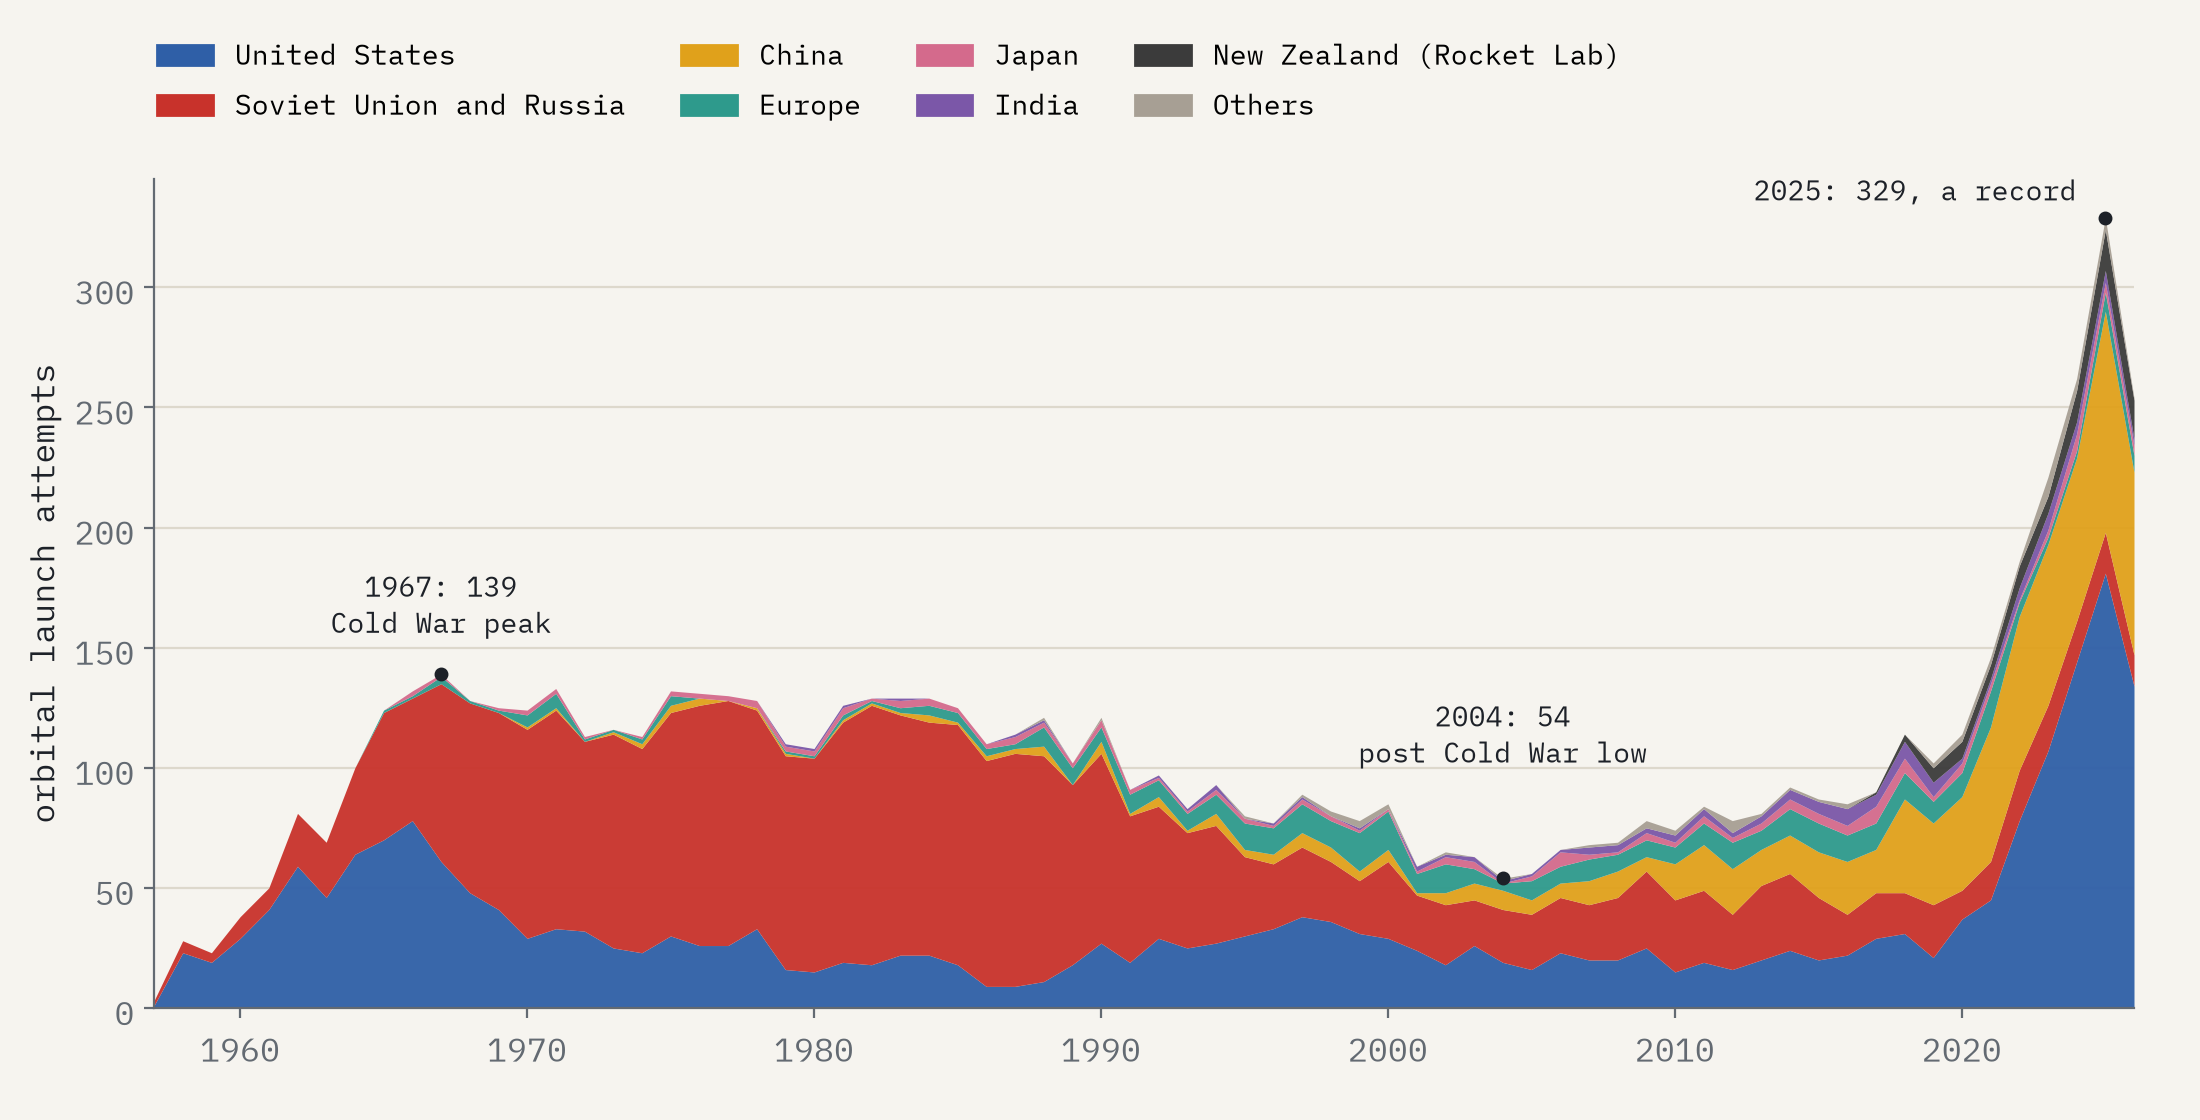
\includegraphics[width=\textwidth]{f_years.png}
\caption{Orbital launch attempts per year, stacked by launching country or bloc as GCAT records it. 2026 is partial.}\label{fig:years}\end{figure}

The recent surge is mostly American and mostly one company. In 2025 the United States made 181 attempts (55\%), 170 of them by SpaceX (165 Falcon 9 flights), of which 122 carried Starlink satellites. China made 92 (28\%) and Russia 17. The number of catalogued payloads launched in 2025 was 4,511, against 218 in 1990. Table~\ref{tab:blocs} summarises each bloc.

\subsection{Failures}
507 attempts (6.8\%) failed. The rate fell from 57\% in 1957 to 1959 and 16\% in the 1960s to 4.2\% in the 1980s and has stayed between about 4\% and 6\% a decade since; the 2020s so far stand at 4.1\% (Figure~\ref{fig:fail}). Because launches are so much more frequent, the number of failures per year in the 2020s (11 in 2025) is higher than at any time since the early 1970s. By bloc, the smaller launching states grouped as others have lost 43\% of their 60 attempts, Japan 13\% and India 12\%, against 7.0\% for the United States and 6.2\% for the Soviet Union and Russia.

\begin{figure}[tbp]\centering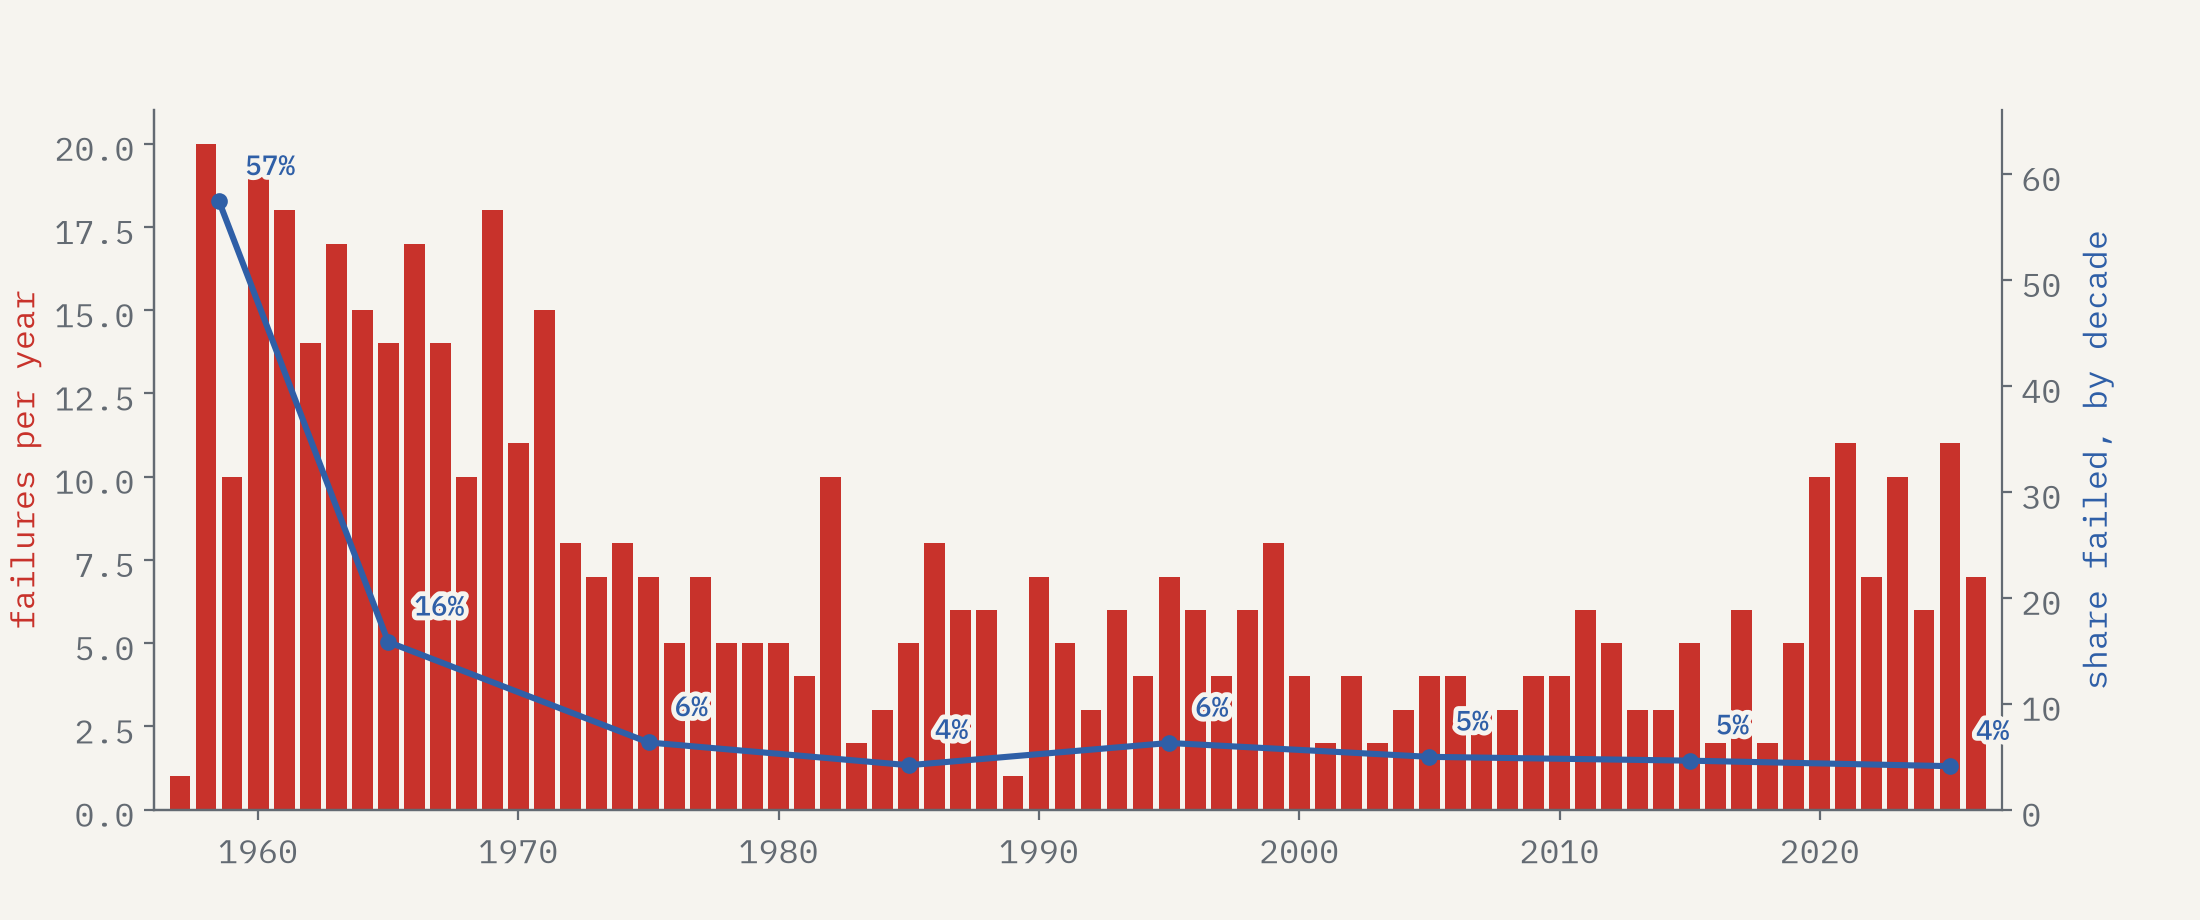
\includegraphics[width=\textwidth]{f_fail.png}
\caption{Launch failures per year (bars) and the share of attempts that failed in each decade (line).}\label{fig:fail}\end{figure}

\subsection{Spaceports}
Figure~\ref{fig:map} maps the 46 spaceports and Table~\ref{tab:ports} lists the busiest. Plesetsk leads with 1,686 attempts, 1,381 of them before 1992, ahead of Baikonur (1,558), Cape Canaveral and Kennedy (1,393; 1,106 from Cape Canaveral codes and 282 from Kennedy) and Vandenberg (938). Since 2020 the order has changed completely (Figure~\ref{fig:ports}): Cape Canaveral and Kennedy (452), Vandenberg (236), Jiuquan (178), Xichang (104), Taiyuan (81), Mahia (75) and Wenchang (71), with Baikonur eighth (56) and Plesetsk at 54. 22 spaceports saw at least one attempt in 2025.

\begin{figure}[tbp]\centering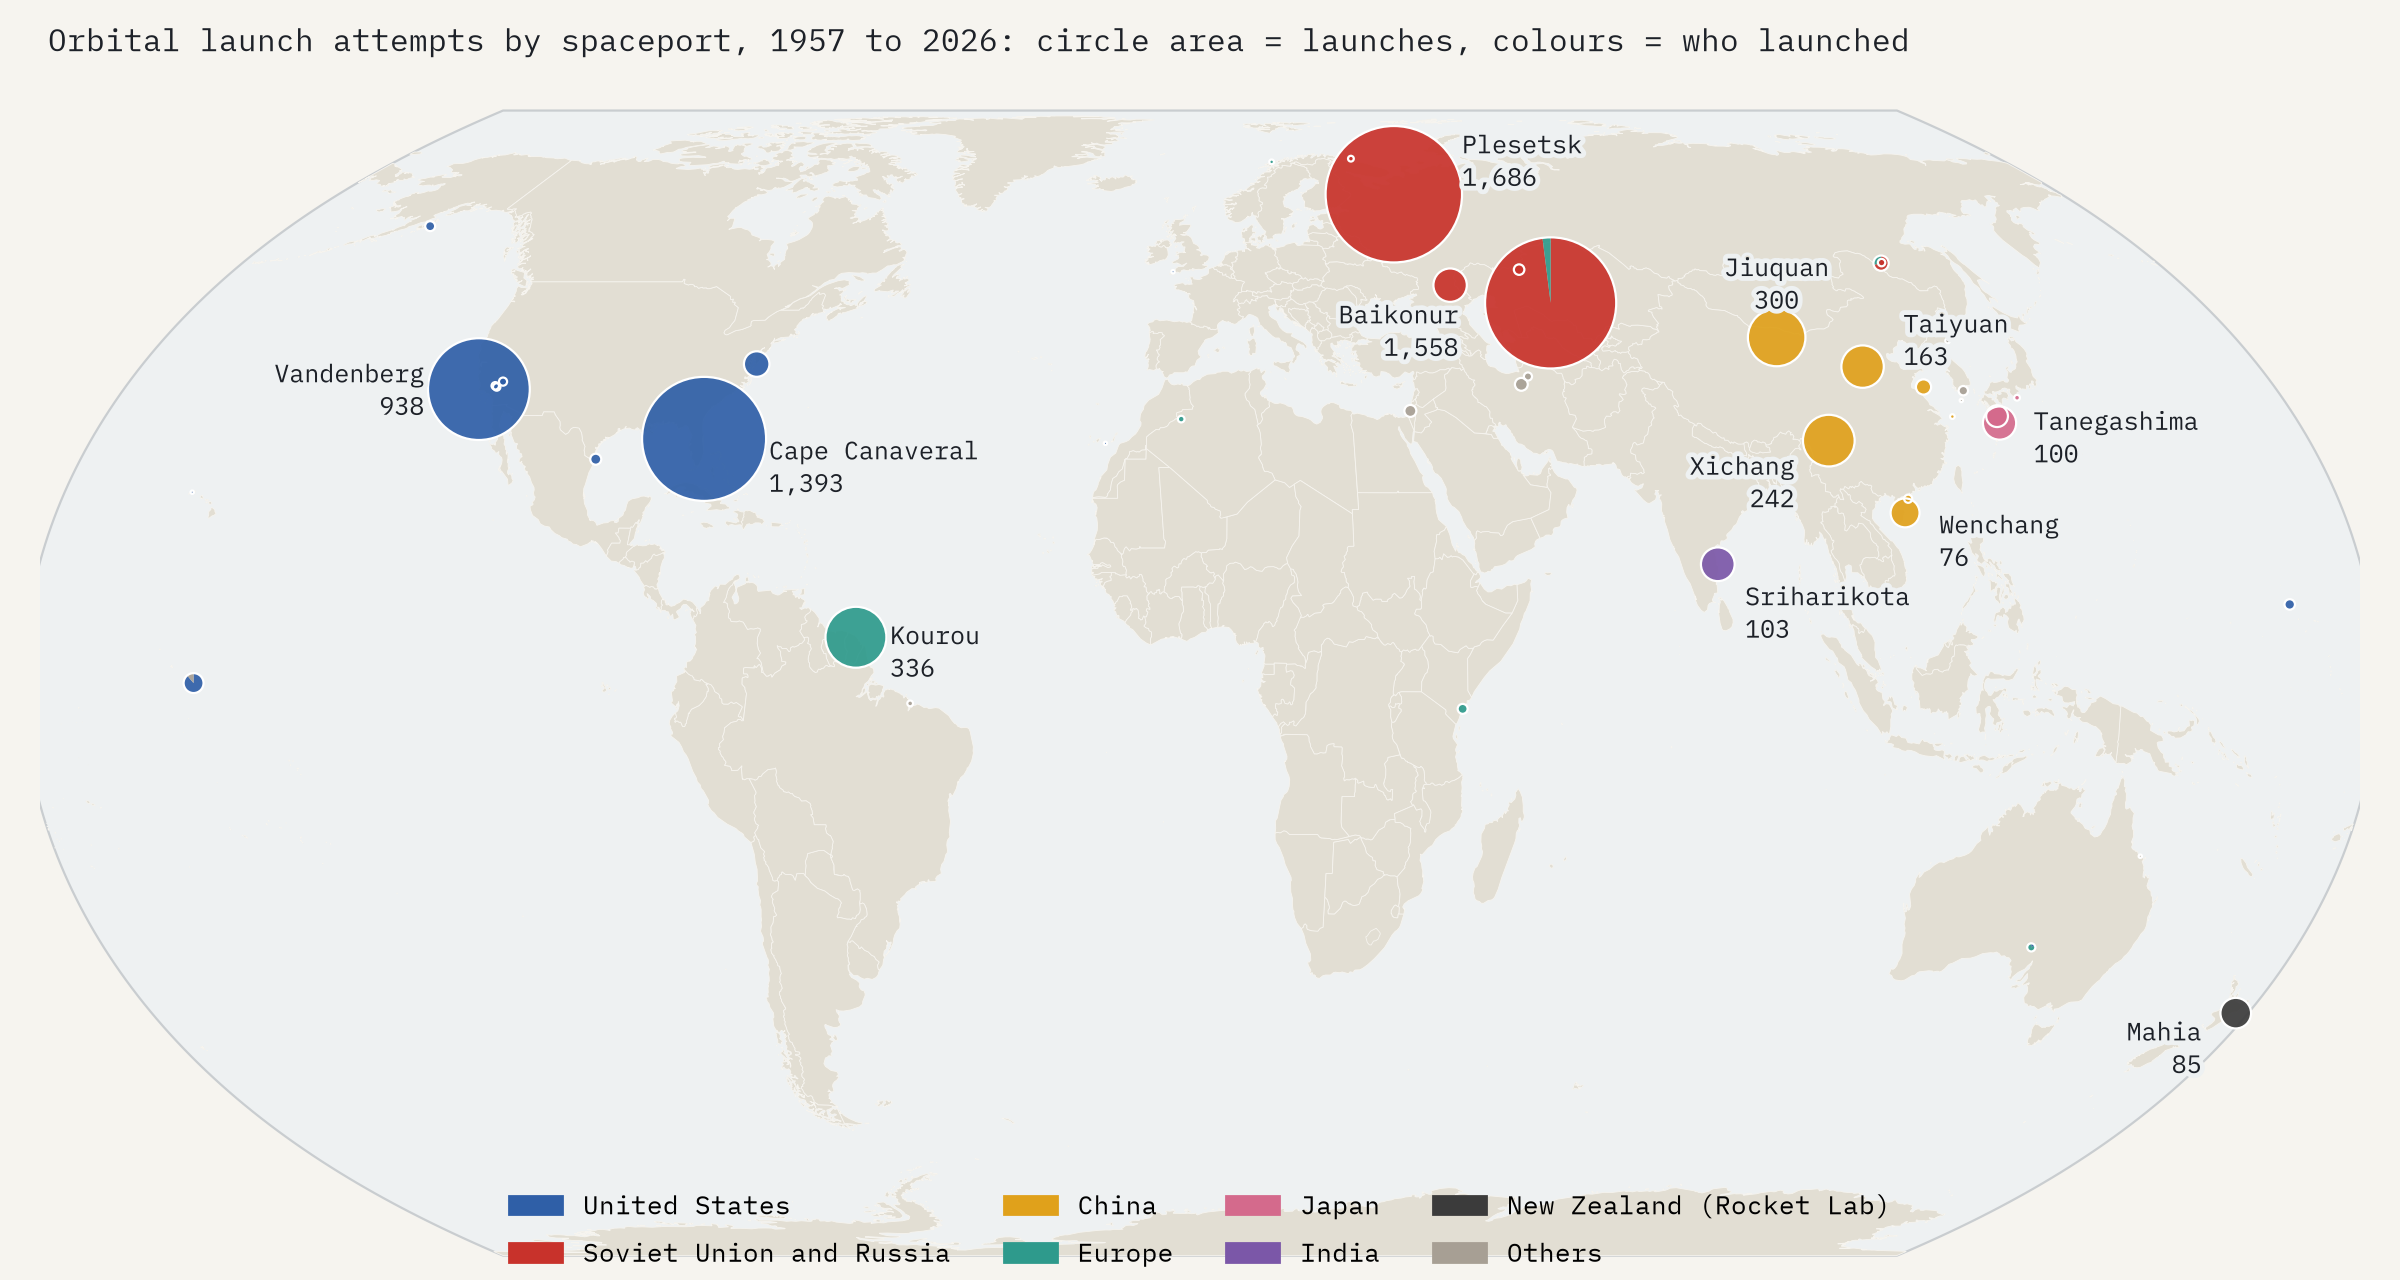
\includegraphics[width=\textwidth]{f_map.png}
\caption{Spaceports, with circle area proportional to orbital launch attempts from 1957 to 2026 and colours showing the launching bloc.}\label{fig:map}\end{figure}

\begin{table}[tbp]\centering\footnotesize\setlength{\tabcolsep}{4pt}\caption{The twenty busiest spaceports: latitude, attempts, failures, first year, busiest year, attempts since 2020 and in 2025.}\label{tab:ports}\begin{tabular}{llrrrrrrr}\toprule Spaceport & Country & Lat. & Attempts & Failed & First & Busiest & 2020+ & 2025\\\midrule
Plesetsk & Russia & 62.9 & 1,686 & 68 & 1966 & 1977 (70) & 54 & 9\\
Baikonur & Kazakhstan & 46.0 & 1,558 & 123 & 1957 & 1987 (48) & 56 & 6\\
Cape Canaveral and Kennedy & United States & 28.5 & 1,393 & 78 & 1957 & 2025 (109) & 452 & 109\\
Vandenberg & United States & 34.6 & 938 & 70 & 1959 & 2026 (69) & 236 & 66\\
Kourou & French Guiana & 5.2 & 336 & 17 & 1970 & 1997 (12) & 39 & 7\\
Jiuquan & China & 41.3 & 300 & 22 & 1970 & 2023 (36) & 178 & 33\\
Xichang & China & 28.2 & 242 & 10 & 1984 & 2024 (19) & 104 & 19\\
Taiyuan & China & 37.5 & 163 & 6 & 1988 & 2022 (14) & 81 & 12\\
Sriharikota & India & 13.6 & 103 & 12 & 1979 & 2016 (7) & 29 & 5\\
Kapustin Yar & Russia & 48.5 & 101 & 16 & 1961 & 1965 (10) & 0 & 0\\
Tanegashima & Japan & 30.4 & 100 & 6 & 1975 & 2017 (6) & 21 & 4\\
Mahia & New Zealand & -39.3 & 85 & 4 & 2017 & 2025 (17) & 75 & 17\\
Wenchang & China & 19.6 & 76 & 3 & 2016 & 2025 (21) & 71 & 21\\
Wallops & United States & 37.8 & 59 & 5 & 1960 & 2013 (4) & 14 & 1\\
Uchinoura & Japan & 31.2 & 43 & 10 & 1966 & 1966 (2) & 2 & 0\\
Sea Launch, Pacific & International waters & 0.0 & 36 & 3 & 1999 & 2006 (5) & 0 & 0\\
Vostochny & Russia & 51.7 & 21 & 1 & 2016 & 2021 (5) & 16 & 2\\
Yellow Sea launches & International waters & 34.9 & 21 & 0 & 2019 & 2025 (7) & 20 & 7\\
Semnan & Iran & 35.2 & 15 & 9 & 2008 & 2012 (3) & 6 & 1\\
Palmachim & Israel & 31.9 & 13 & 2 & 1988 & 1988 (1) & 3 & 1\\
\bottomrule\end{tabular}\end{table}

\begin{figure}[tbp]\centering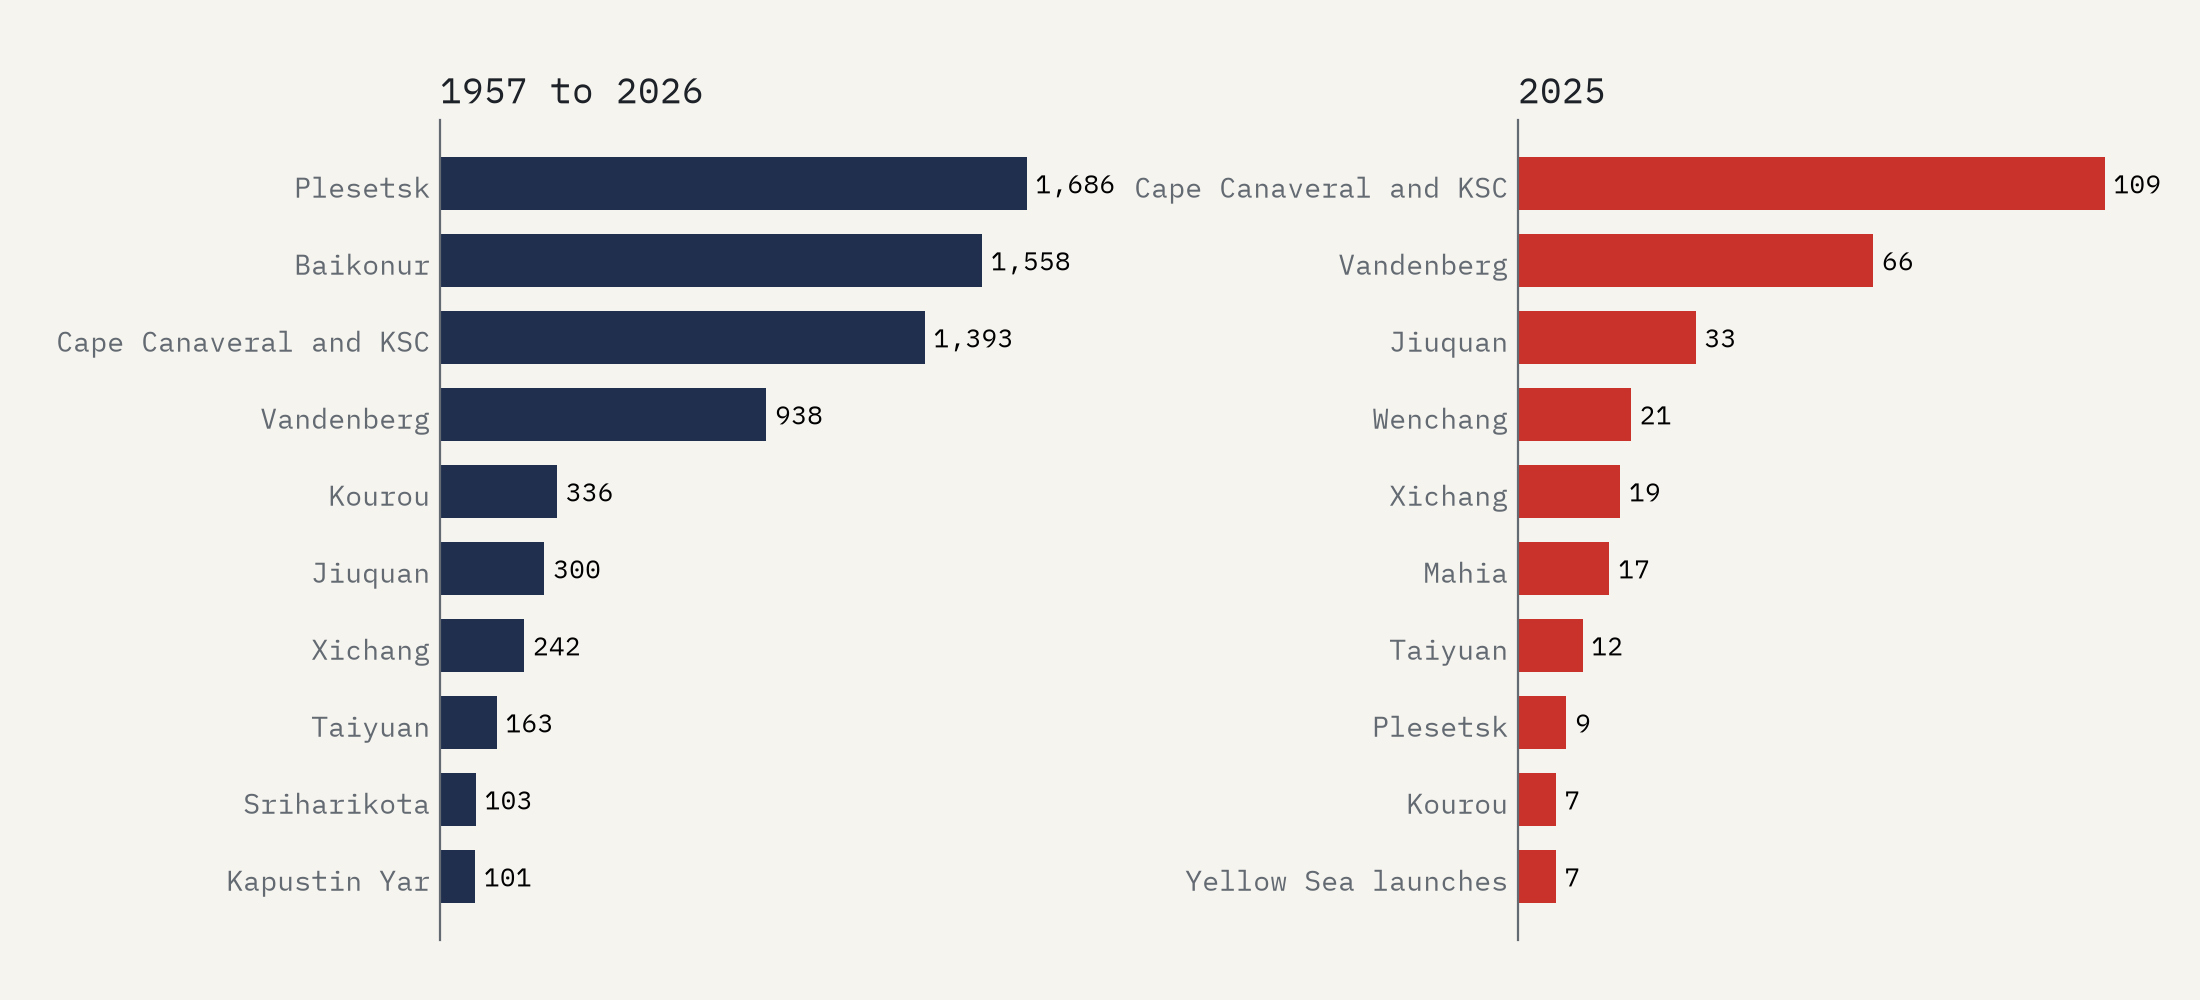
\includegraphics[width=\textwidth]{f_ports.png}
\caption{The busiest spaceports over the whole period (left) and in 2025 (right).}\label{fig:ports}\end{figure}

\subsection{Latitude and direction}
Figure~\ref{fig:lat} orders the main spaceports by latitude. The Earth's rotation gives a rocket 463 m/s at Kourou, 409 m/s at Cape Canaveral, 323 m/s at Baikonur and 212 m/s at Plesetsk, a difference of 140 m/s between Kourou and Baikonur. The more important effect is on inclination: a rocket's orbit is inclined to the equator by at least the latitude of its site unless it spends propellant changing plane, and a geostationary satellite must end with no inclination at all. The share of each site's launches bound for geostationary transfer or geostationary orbit follows latitude: 70\% at Kourou, 27\% at Cape Canaveral and Kennedy, 18\% at Baikonur and 0.2\% at Plesetsk, from where the Soviet Union served high latitudes with Molniya orbits instead.

Direction also reflects where spent stages can fall. Of 5,266 successful launches to low and medium orbits with a known inclination, 65\% went eastward, 33\% into polar or sun-synchronous orbits and 1.4\% westward. The Cape sends 97\% of such launches east over the Atlantic; Vandenberg 68\% south over the Pacific into polar orbits; Israel's Palmachim sends all of its launches west over the Mediterranean, against the Earth's rotation. Only 40 launches (0.8\%) reached an inclination more than two degrees below their site's latitude.

\begin{figure}[tbp]\centering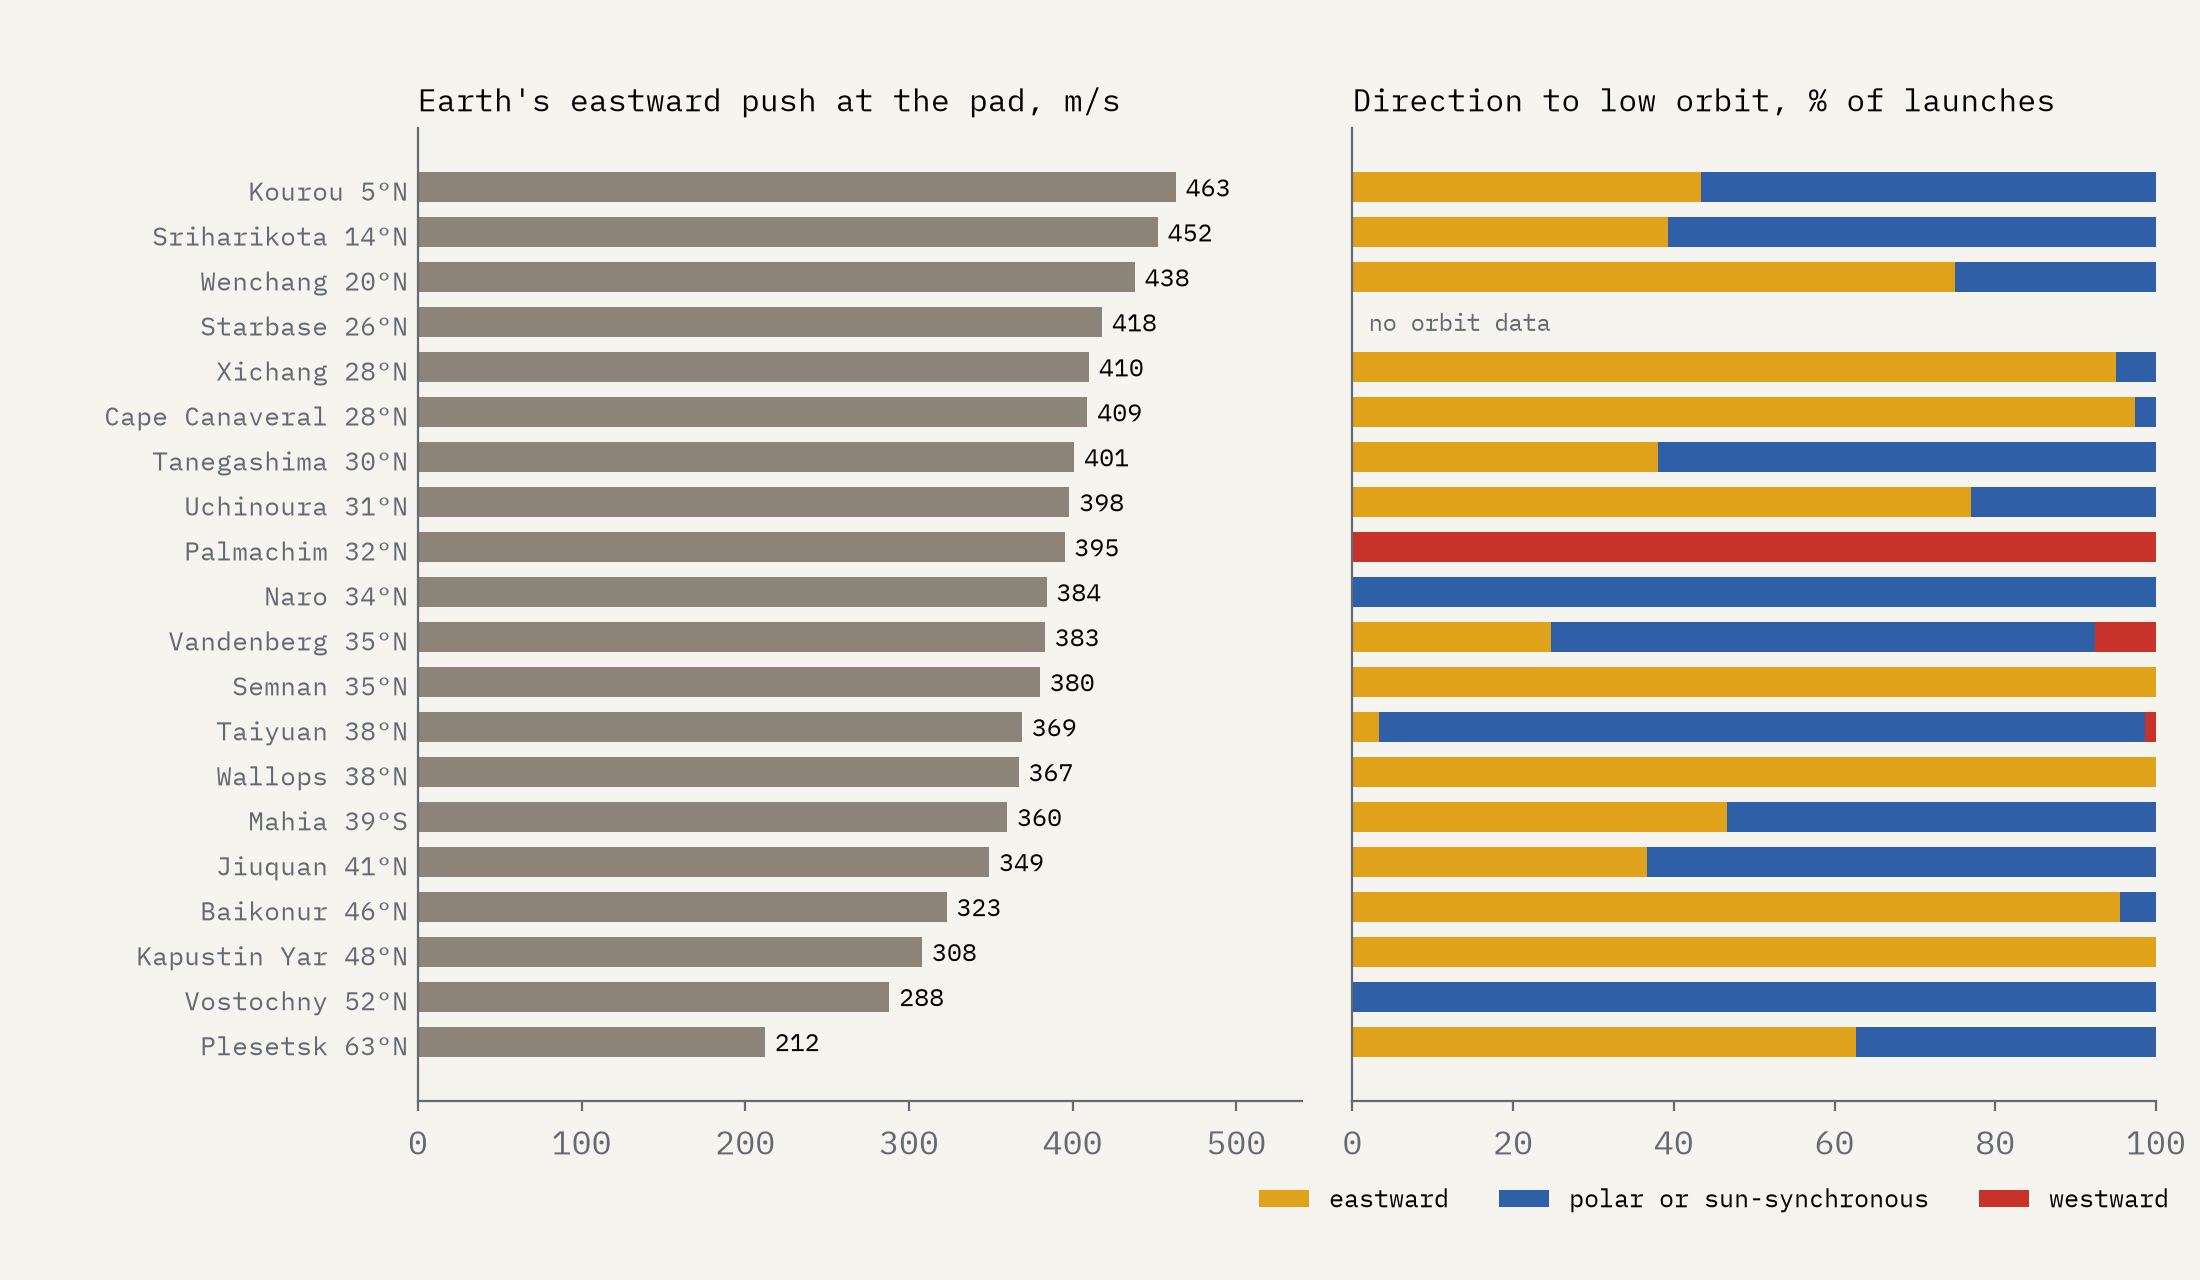
\includegraphics[width=\textwidth]{f_lat.png}
\caption{Spaceports with at least eight launches, by latitude: the eastward speed of the pad (left) and the direction of successful launches to low and medium orbit, from the first payload's inclination (right).}\label{fig:lat}\end{figure}

\subsection{What came back}
Of the 69,999 catalogued objects, 33,397 (48\%) are still in orbit, 10,644 of them Starlink satellites and 34\% debris fragments, and 34,974 (50\%) have come back: 33,715 by uncontrolled re-entry, 1,076 by landing or recovery and 183 (0.5\%) by deliberate deorbit (Figure~\ref{fig:fates}). Those that came back comprise 7,699 payloads, 4,094 rocket stages, 6,517 components and 16,659 debris fragments.

\begin{figure}[tbp]\centering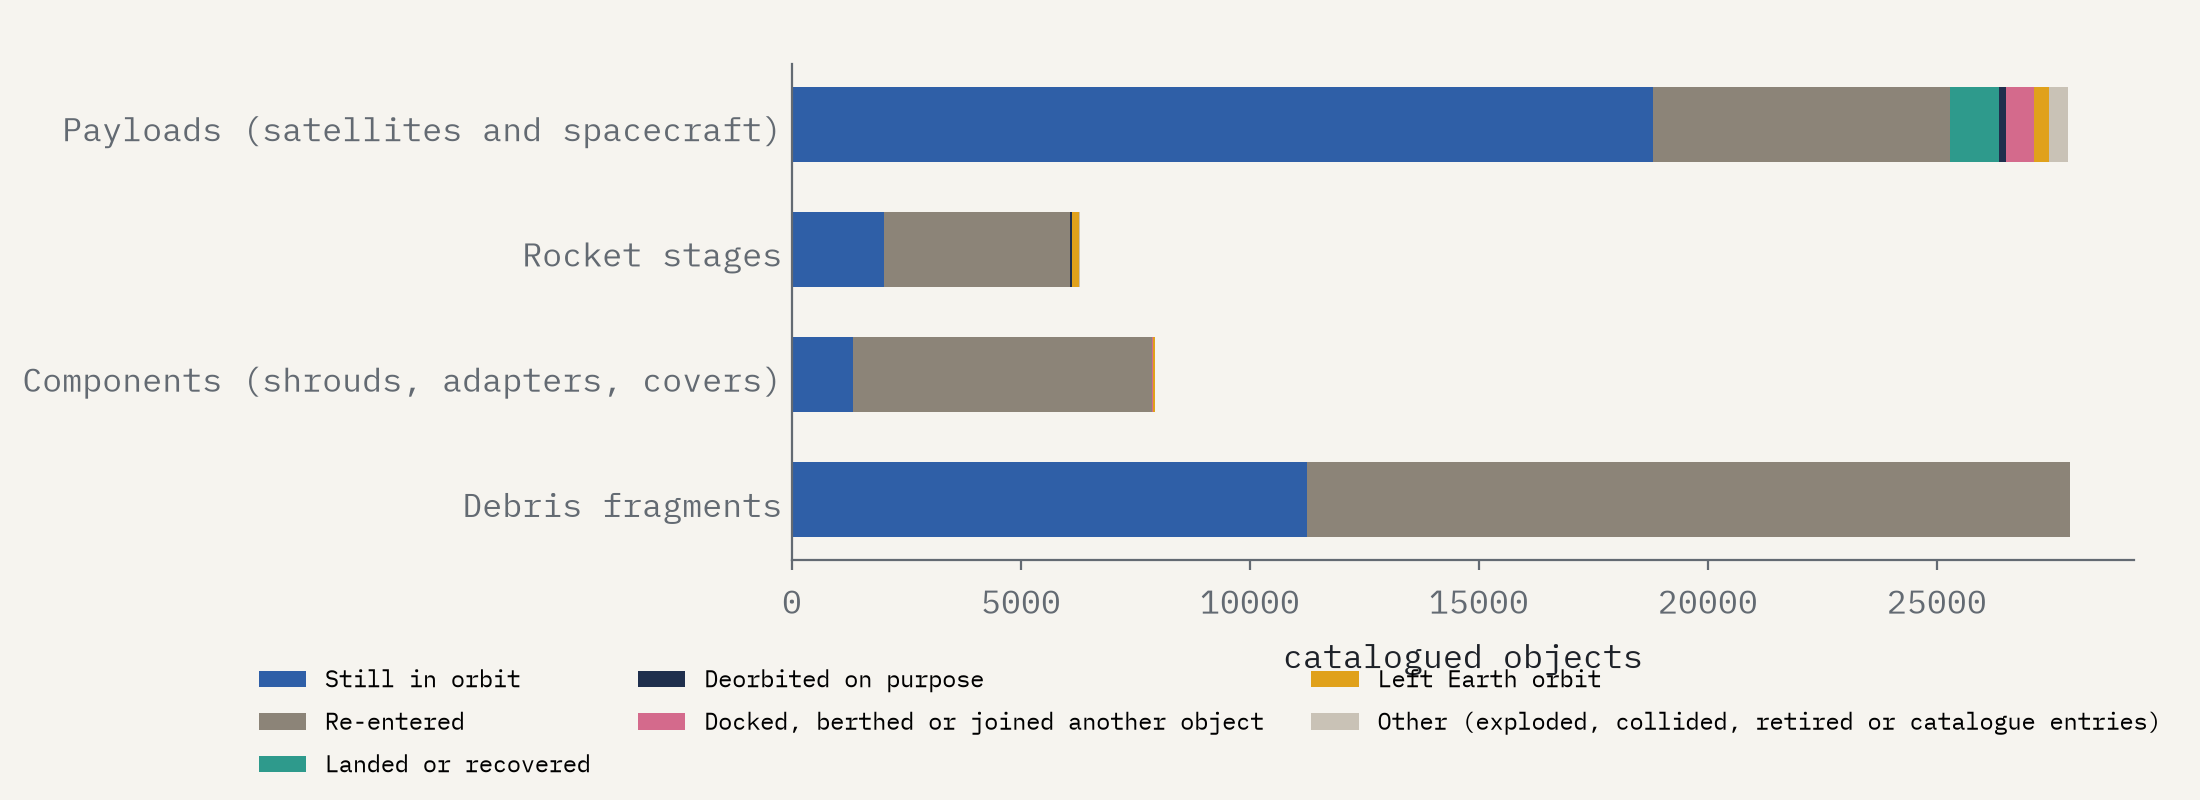
\includegraphics[width=\textwidth]{f_fates.png}
\caption{Catalogued objects by type and fate.}\label{fig:fates}\end{figure}

Returns per year (Figure~\ref{fig:down}) peaked at 2,470 in 2022, of which 1,379 (56\%) were fragments of Kosmos 1408, destroyed in a Russian anti-satellite test in November 2021. In 2025, 1,912 objects came down, 679 (36\%) of them Starlink satellites; in 2019 the figure was 314. 30\% of everything that has ever come back did so in 2020 or later.

\begin{figure}[tbp]\centering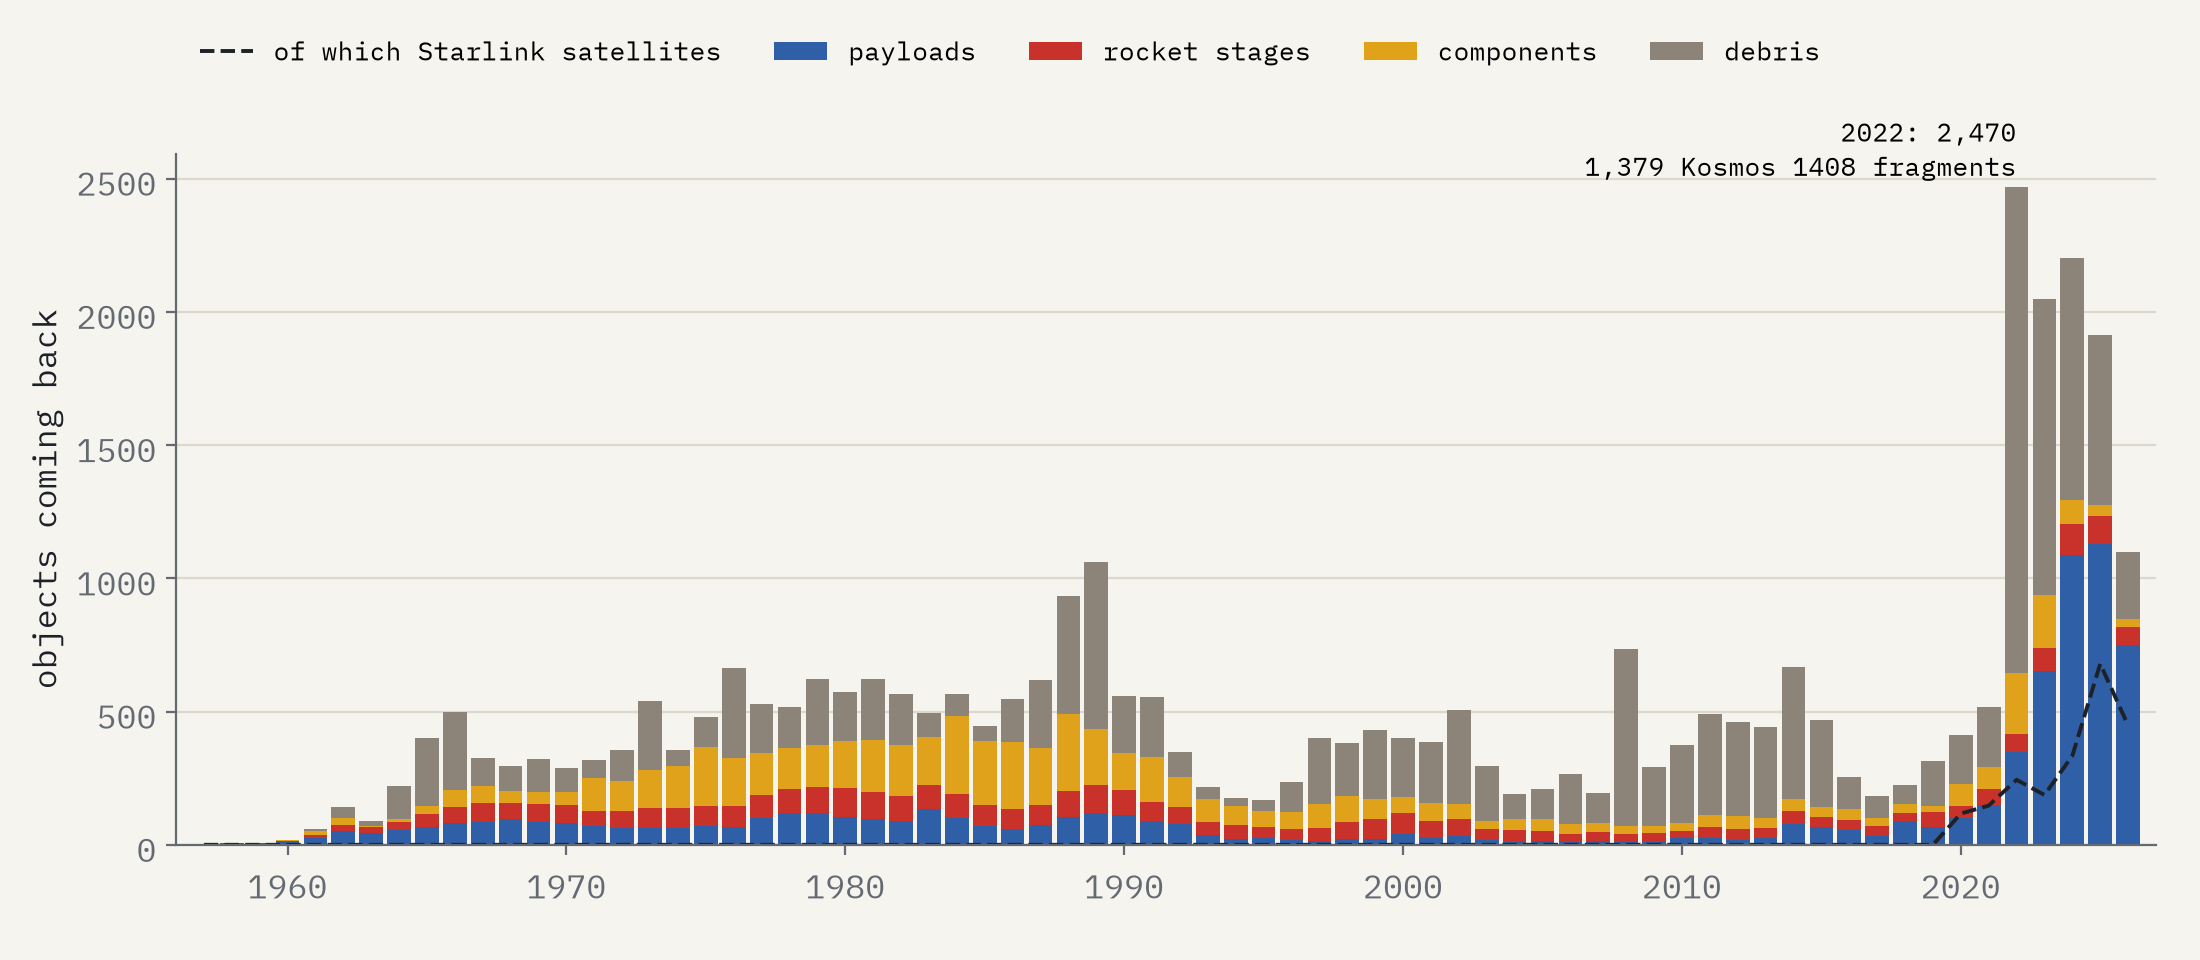
\includegraphics[width=\textwidth]{f_down.png}
\caption{Catalogued objects that re-entered, were deorbited or landed, by year and type. The dashed line counts Starlink satellites.}\label{fig:down}\end{figure}

\subsection{Where things came down}
GCAT records a place as coordinates for 2,136 objects (6.1\% of those that came back), 84\% of them since 2020; another 277 have a place in words only. Among the 2,033 located uncontrolled re-entries, 76\% fall over the sea (Natural Earth 1:50m land), close to the ocean's share of the Earth's surface, and 37\% within the tropics, against 40\% of the surface. 104 (5.1\%) fall within 2,500 km of Point Nemo, 1.35 times the circle's 3.8\% share of the surface; the modest excess is consistent with the latitudes that common orbits cross, and does not suggest that uncontrolled debris is drawn to the cemetery. By contrast, 8 of the 34 located deliberate deorbits fall within the circle (Figure~\ref{fig:reentry}).

\begin{figure}[tbp]\centering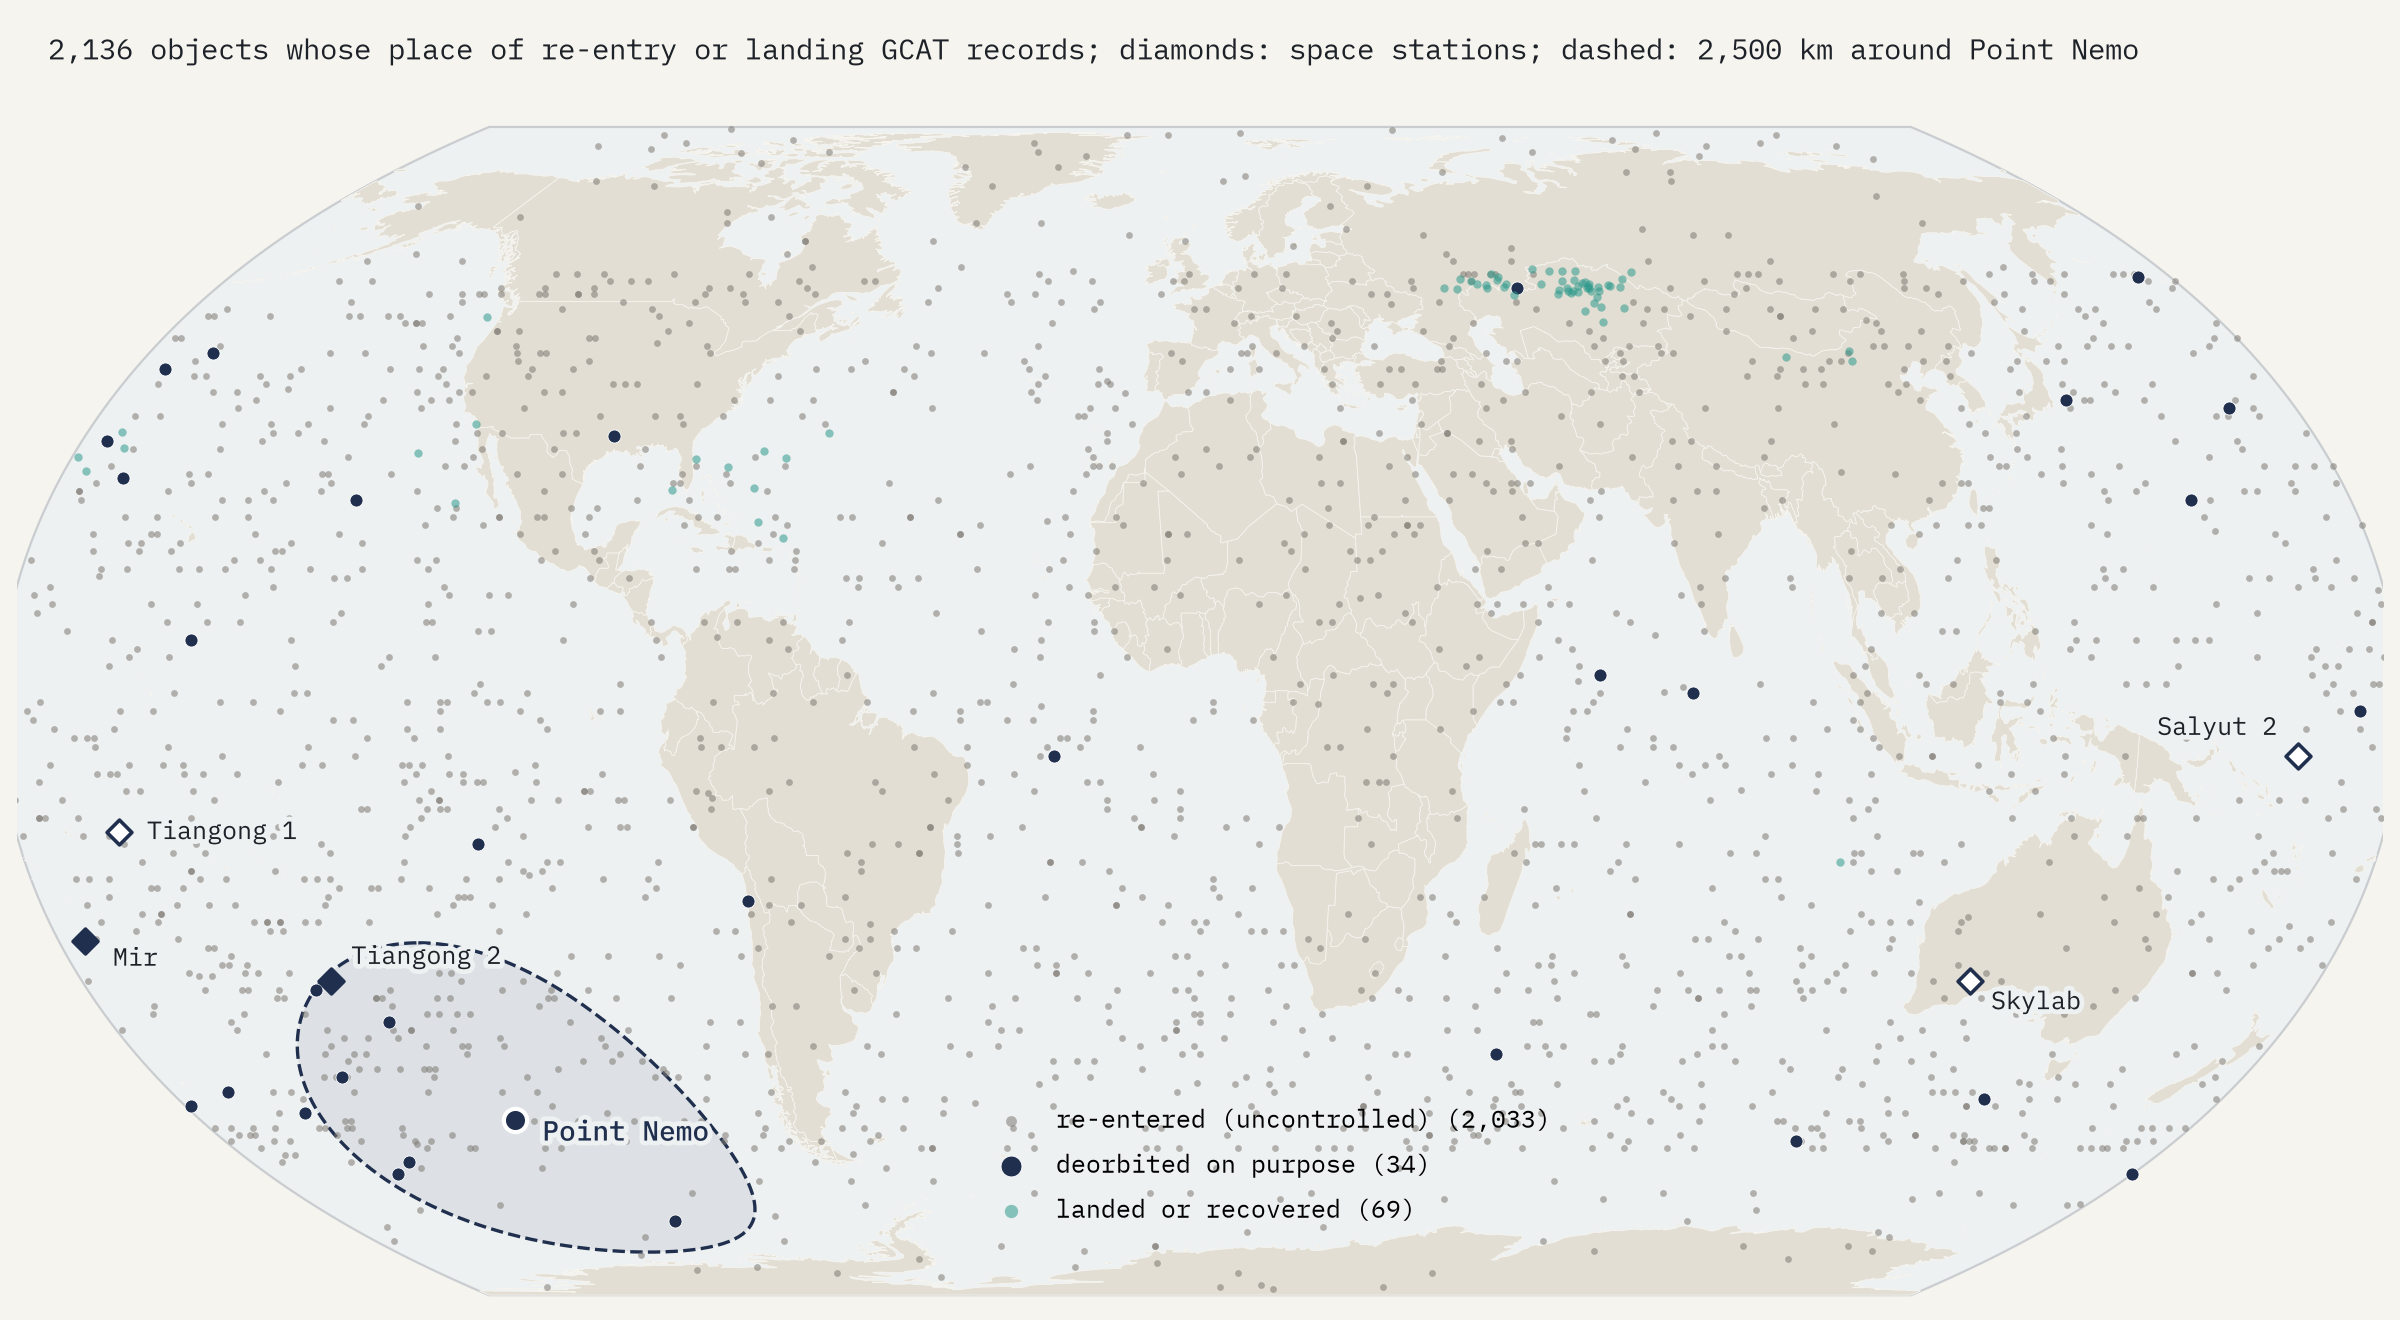
\includegraphics[width=\textwidth]{f_reentry_map.png}
\caption{Objects whose place of re-entry or landing GCAT records, with the space stations and an indicative 2,500 km circle around Point Nemo.}\label{fig:reentry}\end{figure}

\subsection{The spacecraft cemetery}
Point Nemo lies about 2,688 km from the nearest land and was identified by Hrvoje Lukatela in 1992 \citep{wikinemo}. Wikipedia's article on the spacecraft cemetery reports that more than 260 spacecraft were disposed of in the area between 1971 to 2016, nearly 200 pieces of them Russian, including Mir and six Salyut stations and cargo craft such as Progress, the H-II Transfer Vehicle and the Automated Transfer Vehicle \citep{wikicem}. Table~\ref{tab:stations} gives GCAT's record for every station. Salyut 1, 3, 4, 5 and 6 are recorded as deorbited into the Pacific Ocean region; Salyut 2 and Salyut 7 and America's Skylab re-entered without control; Mir was deorbited on 23 March 2001; Tiangong 1 re-entered without control in 2018 and Tiangong 2 was deorbited in 2019. GCAT catalogues 183 Progress ships since 1978, 10 Japanese cargo ships and 5 ATVs. Their final deorbits are recorded in GCAT's event catalogues, which this study does not use, because in the main catalogue their first phase ends when they dock with a station.

\begin{table}[tbp]\centering\small\caption{Space stations in GCAT: launch year, end date, mass (main module), status and recorded place.}\label{tab:stations}\begin{tabular}{lrrrll}\toprule Station & Launched & Came down & Tonnes & Status & GCAT place\\\midrule
Salyut 1 & 1971 & 1971 Oct 11 & 18.2 & deorbited & POR\\
Salyut 2 & 1973 & 1973 May 28 & 18.7 & re-entered & 165E 5S?\\
Salyut 3 & 1974 & 1975 Jan 24 & 18.9 & deorbited & POR\\
Salyut 4 & 1974 & 1977 Feb  2 & 18.5 & deorbited & POR\\
Salyut 5 & 1976 & 1977 Aug  8 & 18.9 & deorbited & POR\\
Salyut 6 & 1977 & 1982 Jul 29 & 19.8 & deorbited & POR\\
Salyut 7 & 1982 & 1991 Feb  7 & 19.8 & re-entered & Argentina\\
Skylab & 1973 & 1979 Jul 11 & 34.0 & re-entered & 31S 124E\\
Mir & 1986 & 2001 Mar 23 & 20.1 & deorbited & 26.22S 175.88W\\
Tiangong 1 & 2011 & 2018 Apr  2 & 8.5 & re-entered & 164.3W 13.6S\\
Tiangong 2 & 2016 & 2019 Jul 19 & 8.6 & deorbited & 140W 31S\\
\bottomrule\end{tabular}\end{table}

\section{Limitations}
First, GCAT is one person's careful compilation, and some classifications (what counts as an orbital attempt, a partial failure or a launching agency) are judgements; I follow them rather than second guess them. Second, the bloc assignment is by agency, not by the nationality of the vehicle or the location of the site, so it can differ from other tallies. Third, the main object catalogue excludes objects that have not yet been given standard catalogue numbers, and debris counts reflect only what can be tracked. Fourth, the fates of objects that docked with another are in the event catalogues, not used here, so deliberate deorbits of cargo craft are not counted. Fifth, the recorded re-entry places are rough, cover only 6\% of returns and are dominated by recent years. Sixth, direction is inferred from the inclination of the first payload, not from launch azimuths. Seventh, 2026 is incomplete.

\section{Conclusion}
Seventy years of orbital launches fall into three eras: a Cold War plateau of more than a hundred launches a year from a handful of military ranges, a post Soviet decline to about one a week, and since 2020 an explosion driven by reusable rockets and satellite constellations that has already doubled the old record. What goes up increasingly comes back: half of everything ever catalogued has fallen, most of it burning up wherever its orbit decayed. Point Nemo is where the largest controlled returns are aimed, and that makes it a symbol of space hardware's end, but in the record it is the exception, not the rule.

\section*{Data and code availability}
The interactive map is at \url{https://maps.tristanhotham.com/rocket-launches/}. Data and code are at \url{https://github.com/Tristan-Hotham/rocket-launches} and archived with this paper at https://doi.org/10.5281/zenodo.23857612. Derived data are released under CC BY 4.0 and code under the MIT licence. Launch and object data: GCAT (J. McDowell, planet4589.org/space/gcat), CC BY 4.0.

\section*{AI statement}
I wrote the text, with drafting and editing assistance from Claude (Anthropic), which also helped prepare the analysis code. I reviewed and checked all text and results.

\begin{thebibliography}{9}
\bibitem[McDowell(2020)]{gcat} McDowell, J. C. (2020) General Catalog of Artificial Space Objects, release 1.8.8. CC BY 4.0. \url{https://planet4589.org/space/gcat}
\bibitem[Natural Earth(2026)]{naturalearth} Natural Earth (2026) Admin 0 countries, land and populated places, 1:50m and 1:10m. Public domain. \url{https://www.naturalearthdata.com/}
\bibitem[Wikipedia(2026a)]{wikinemo} Wikipedia contributors (2026) Pole of inaccessibility (revision 1381723518). CC BY-SA 4.0. \url{https://en.wikipedia.org/wiki/Pole_of_inaccessibility}
\bibitem[Wikipedia(2026b)]{wikicem} Wikipedia contributors (2026) Spacecraft cemetery (revision 1380647807). CC BY-SA 4.0. \url{https://en.wikipedia.org/wiki/Spacecraft_cemetery}
\bibitem[Wikipedia(2026c)]{wikiport} Wikipedia contributors (2026) Spaceport (revision 1381738622). CC BY-SA 4.0. \url{https://en.wikipedia.org/wiki/Spaceport}
\bibitem[Wikipedia(2026d)]{wikilist} Wikipedia contributors (2026) List of rocket launch sites (revision 1373883742). CC BY-SA 4.0. \url{https://en.wikipedia.org/wiki/List_of_rocket_launch_sites}
\end{thebibliography}
\end{document}
